\documentclass[a4paper]{book}
\usepackage{makeidx}
\usepackage{natbib}
\usepackage{graphicx}
\usepackage{multicol}
\usepackage{float}
\usepackage{listings}
\usepackage{color}
\usepackage{ifthen}
\usepackage[table]{xcolor}
\usepackage{textcomp}
\usepackage{alltt}
\usepackage{ifpdf}
\ifpdf
\usepackage[pdftex,
            pagebackref=true,
            colorlinks=true,
            linkcolor=blue,
            unicode
           ]{hyperref}
\else
\usepackage[ps2pdf,
            pagebackref=true,
            colorlinks=true,
            linkcolor=blue,
            unicode
           ]{hyperref}
\usepackage{pspicture}
\fi
\usepackage[utf8]{inputenc}
\usepackage{mathptmx}
\usepackage[scaled=.90]{helvet}
\usepackage{courier}
\usepackage{sectsty}
\usepackage[titles]{tocloft}
\usepackage{doxygen}
\lstset{language=C++,inputencoding=utf8,basicstyle=\footnotesize,breaklines=true,breakatwhitespace=true,tabsize=8,numbers=left }
\makeindex
\setcounter{tocdepth}{3}
\renewcommand{\footrulewidth}{0.4pt}
\renewcommand{\familydefault}{\sfdefault}
\hfuzz=15pt
\setlength{\emergencystretch}{15pt}
\hbadness=750
\tolerance=750
\begin{document}
\hypersetup{pageanchor=false,citecolor=blue}
\begin{titlepage}
\vspace*{7cm}
\begin{center}
{\Large \-L\-R\-T \\[1ex]\large 12 }\\
\vspace*{1cm}
{\large \-Generated by Doxygen 1.7.6.1}\\
\vspace*{0.5cm}
{\small Fri Jan 20 2012 17:02:04}\\
\end{center}
\end{titlepage}
\clearemptydoublepage
\pagenumbering{roman}
\tableofcontents
\clearemptydoublepage
\pagenumbering{arabic}
\hypersetup{pageanchor=true,citecolor=blue}
\chapter{\-Class \-Index}
\section{\-Class \-Hierarchy}
\-This inheritance list is sorted roughly, but not completely, alphabetically\-:\begin{DoxyCompactList}
\item \contentsline{section}{\-Action\-Data}{\pageref{class_action_data}}{}
\item \contentsline{section}{\-Asynchronous\-Printer}{\pageref{class_asynchronous_printer}}{}
\item \contentsline{section}{\-Brain}{\pageref{class_brain}}{}
\item \contentsline{section}{\-Build}{\pageref{class_build}}{}
\item \contentsline{section}{\-Component}{\pageref{class_component}}{}
\item \contentsline{section}{\-Component\-Data}{\pageref{struct_component_data}}{}
\item \contentsline{section}{\-Config}{\pageref{class_config}}{}
\item \contentsline{section}{\-Configurable}{\pageref{class_configurable}}{}
\item \contentsline{section}{\-Config\-Val}{\pageref{struct_config_val}}{}
\item \contentsline{section}{\-Console}{\pageref{class_console}}{}
\item \contentsline{section}{\-Driver\-Station\-Config}{\pageref{class_driver_station_config}}{}
\item \contentsline{section}{\-L\-C\-D}{\pageref{class_l_c_d}}{}
\item \contentsline{section}{\-L\-R\-T\-Robot\-Base}{\pageref{class_l_r_t_robot_base}}{}
\begin{DoxyCompactList}
\item \contentsline{section}{\-L\-R\-T\-Robot12}{\pageref{class_l_r_t_robot12}}{}
\end{DoxyCompactList}
\item \contentsline{section}{\-Print\-In\-Constructor}{\pageref{class_print_in_constructor}}{}
\item \contentsline{section}{\-Profiled\-Section}{\pageref{class_profiled_section}}{}
\item \contentsline{section}{\-Profiler}{\pageref{class_profiler}}{}
\item \contentsline{section}{\-Profiler\-Helper}{\pageref{class_profiler_helper}}{}
\item \contentsline{section}{\-Running\-Sum}{\pageref{class_running_sum}}{}
\item \contentsline{section}{\-Sort\-By\-Second\-Value$<$ \-Pair\-T $>$}{\pageref{struct_sort_by_second_value}}{}
\item \contentsline{section}{\-Util}{\pageref{class_util}}{}
\end{DoxyCompactList}

\chapter{\-Class \-Index}
\section{\-Class \-List}
\-Here are the classes, structs, unions and interfaces with brief descriptions\-:\begin{DoxyCompactList}
\item\contentsline{section}{\hyperlink{class_action_data}{\-Action\-Data} \\*\-Contains the actionable data (ex. setpoints) for the components }{\pageref{class_action_data}}{}
\item\contentsline{section}{\hyperlink{class_asynchronous_printer}{\-Asynchronous\-Printer} \\*\-Provides an asynchronous equivilent of printf }{\pageref{class_asynchronous_printer}}{}
\item\contentsline{section}{\hyperlink{class_brain}{\-Brain} \\*\-Processes inputs from \{\-Autonomous$|$\-Joystick\} and sets appropriate values in \hyperlink{class_action_data}{\-Action\-Data} }{\pageref{class_brain}}{}
\item\contentsline{section}{\hyperlink{class_build}{\-Build} \\*\-Class that contains the build time and build number }{\pageref{class_build}}{}
\item\contentsline{section}{\hyperlink{class_component}{\-Component} }{\pageref{class_component}}{}
\item\contentsline{section}{\hyperlink{struct_component_data}{\-Component\-Data} }{\pageref{struct_component_data}}{}
\item\contentsline{section}{\hyperlink{class_config}{\-Config} \\*\-A \-Singleton that stores and retrieves configuration values from a file }{\pageref{class_config}}{}
\item\contentsline{section}{\hyperlink{class_configurable}{\-Configurable} \\*\-The base class for all classes that read values from the configuration system }{\pageref{class_configurable}}{}
\item\contentsline{section}{\hyperlink{struct_config_val}{\-Config\-Val} }{\pageref{struct_config_val}}{}
\item\contentsline{section}{\hyperlink{class_console}{\-Console} }{\pageref{class_console}}{}
\item\contentsline{section}{\hyperlink{class_driver_station_config}{\-Driver\-Station\-Config} }{\pageref{class_driver_station_config}}{}
\item\contentsline{section}{\hyperlink{class_l_c_d}{\-L\-C\-D} }{\pageref{class_l_c_d}}{}
\item\contentsline{section}{\hyperlink{class_l_r_t_robot12}{\-L\-R\-T\-Robot12} }{\pageref{class_l_r_t_robot12}}{}
\item\contentsline{section}{\hyperlink{class_l_r_t_robot_base}{\-L\-R\-T\-Robot\-Base} }{\pageref{class_l_r_t_robot_base}}{}
\item\contentsline{section}{\hyperlink{class_print_in_constructor}{\-Print\-In\-Constructor} }{\pageref{class_print_in_constructor}}{}
\item\contentsline{section}{\hyperlink{class_profiled_section}{\-Profiled\-Section} }{\pageref{class_profiled_section}}{}
\item\contentsline{section}{\hyperlink{class_profiler}{\-Profiler} }{\pageref{class_profiler}}{}
\item\contentsline{section}{\hyperlink{class_profiler_helper}{\-Profiler\-Helper} }{\pageref{class_profiler_helper}}{}
\item\contentsline{section}{\hyperlink{class_running_sum}{\-Running\-Sum} }{\pageref{class_running_sum}}{}
\item\contentsline{section}{\hyperlink{struct_sort_by_second_value}{\-Sort\-By\-Second\-Value$<$ Pair\-T $>$} }{\pageref{struct_sort_by_second_value}}{}
\item\contentsline{section}{\hyperlink{class_util}{\-Util} }{\pageref{class_util}}{}
\end{DoxyCompactList}

\chapter{\-Class \-Documentation}
\hypertarget{class_action_data}{\section{\-Action\-Data \-Class \-Reference}
\label{class_action_data}\index{\-Action\-Data@{\-Action\-Data}}
}


\-Contains the actionable data (ex. setpoints) for the components.  




{\ttfamily \#include $<$\-Action\-Data.\-h$>$}



\subsection{\-Detailed \-Description}
\-Contains the actionable data (ex. setpoints) for the components. 

\begin{DoxyAuthor}{\-Author}
\-Brian \-Axelrod 

\-Robert \-Ying 
\end{DoxyAuthor}


\-The documentation for this class was generated from the following file\-:\begin{DoxyCompactItemize}
\item 
\-Action\-Data/\-Action\-Data.\-h\end{DoxyCompactItemize}

\hypertarget{class_asynchronous_printer}{\section{\-Asynchronous\-Printer \-Class \-Reference}
\label{class_asynchronous_printer}\index{\-Asynchronous\-Printer@{\-Asynchronous\-Printer}}
}


\-Provides an asynchronous equivilent of printf.  




{\ttfamily \#include $<$\-Asynchronous\-Printer.\-h$>$}

\subsection*{\-Static \-Public \-Member \-Functions}
\begin{DoxyCompactItemize}
\item 
\hypertarget{class_asynchronous_printer_ab1553ae0b41d933f38a8e8439f687b42}{static \hyperlink{class_asynchronous_printer}{\-Asynchronous\-Printer} \& {\bfseries \-Instance} ()}\label{class_asynchronous_printer_ab1553ae0b41d933f38a8e8439f687b42}

\item 
\hypertarget{class_asynchronous_printer_a0ef1c5904f24fd48fda1e724f4f0f68f}{static int \hyperlink{class_asynchronous_printer_a0ef1c5904f24fd48fda1e724f4f0f68f}{\-Printf} (const char $\ast$format,...)}\label{class_asynchronous_printer_a0ef1c5904f24fd48fda1e724f4f0f68f}

\begin{DoxyCompactList}\small\item\em \-Asynchronous alternative to \-Printf. \end{DoxyCompactList}\item 
\hypertarget{class_asynchronous_printer_af42d841d7d5c70f34e81c98a212478b6}{static void {\bfseries \-Quit} ()}\label{class_asynchronous_printer_af42d841d7d5c70f34e81c98a212478b6}

\item 
\hypertarget{class_asynchronous_printer_af56a3f2c43c68f55495fc7ffd1025c1e}{static bool {\bfseries \-Queue\-Empty} ()}\label{class_asynchronous_printer_af56a3f2c43c68f55495fc7ffd1025c1e}

\end{DoxyCompactItemize}


\subsection{\-Detailed \-Description}
\-Provides an asynchronous equivilent of printf. 

\-The documentation for this class was generated from the following files\-:\begin{DoxyCompactItemize}
\item 
\-Util/\-Asynchronous\-Printer.\-h\item 
\-Util/\-Asynchronous\-Printer.\-cpp\end{DoxyCompactItemize}

\hypertarget{class_brain}{\section{\-Brain \-Class \-Reference}
\label{class_brain}\index{\-Brain@{\-Brain}}
}


\-Processes inputs from \{\-Autonomous$|$\-Joystick\} and sets appropriate values in \hyperlink{class_action_data}{\-Action\-Data}.  




{\ttfamily \#include $<$\-Brain.\-h$>$}



\subsection{\-Detailed \-Description}
\-Processes inputs from \{\-Autonomous$|$\-Joystick\} and sets appropriate values in \hyperlink{class_action_data}{\-Action\-Data}. 

\begin{DoxyAuthor}{\-Author}
\-Brian \-Axelrod 

\-Robert \-Ying 
\end{DoxyAuthor}


\-The documentation for this class was generated from the following file\-:\begin{DoxyCompactItemize}
\item 
\-Brain/\-Brain.\-h\end{DoxyCompactItemize}

\hypertarget{class_build}{\section{\-Build \-Class \-Reference}
\label{class_build}\index{\-Build@{\-Build}}
}


the class that contains the build time and build number.  




{\ttfamily \#include $<$\-Build.\-h$>$}

\subsection*{\-Static \-Public \-Member \-Functions}
\begin{DoxyCompactItemize}
\item 
\hypertarget{class_build_a9f5d52e1840e568016036c34124da091}{static int \hyperlink{class_build_a9f5d52e1840e568016036c34124da091}{\-Get\-Number} ()}\label{class_build_a9f5d52e1840e568016036c34124da091}

\begin{DoxyCompactList}\small\item\em public accessor for the build number. \end{DoxyCompactList}\item 
\hypertarget{class_build_a129bada4f288e35d2340e157f6414c1f}{static std\-::string \hyperlink{class_build_a129bada4f288e35d2340e157f6414c1f}{\-Get\-Time} ()}\label{class_build_a129bada4f288e35d2340e157f6414c1f}

\begin{DoxyCompactList}\small\item\em \-Public accessor for the time of the last build. \end{DoxyCompactList}\end{DoxyCompactItemize}


\subsection{\-Detailed \-Description}
the class that contains the build time and build number. 

\-The documentation for this class was generated from the following files\-:\begin{DoxyCompactItemize}
\item 
\-Config/\-Build.\-h\item 
\-Config/\-Build.\-cpp\end{DoxyCompactItemize}

\hypertarget{class_component}{\section{\-Component \-Class \-Reference}
\label{class_component}\index{\-Component@{\-Component}}
}
\subsection*{\-Public \-Member \-Functions}
\begin{DoxyCompactItemize}
\item 
\hypertarget{class_component_a7d4181cf107d1aee4128dc1c3670d120}{virtual void \hyperlink{class_component_a7d4181cf107d1aee4128dc1c3670d120}{\-Output} ()=0}\label{class_component_a7d4181cf107d1aee4128dc1c3670d120}

\begin{DoxyCompactList}\small\item\em called every time the main loop iterates. \end{DoxyCompactList}\item 
\hypertarget{class_component_a66794e7955105c819bb50c0cf0073192}{virtual string \hyperlink{class_component_a66794e7955105c819bb50c0cf0073192}{\-Get\-Name} ()=0}\label{class_component_a66794e7955105c819bb50c0cf0073192}

\begin{DoxyCompactList}\small\item\em returns the name of the component which is helpful for debugging and profiling. \end{DoxyCompactList}\end{DoxyCompactItemize}
\subsection*{\-Static \-Public \-Member \-Functions}
\begin{DoxyCompactItemize}
\item 
static list$<$ \-Component\-With\-Data $>$ $\ast$ \hyperlink{class_component_ab6f5ceb93adde86d8f93beb42cccb832}{\-Create\-Components} ()
\begin{DoxyCompactList}\small\item\em the \-Factory method that constructs all the components. \-This makes it so that the main loop does not have to know about the individual components. \end{DoxyCompactList}\end{DoxyCompactItemize}
\subsection*{\-Protected \-Attributes}
\begin{DoxyCompactItemize}
\item 
\hyperlink{class_action_data}{\-Action\-Data} $\ast$ \hyperlink{class_component_a16168a59f8d8e139632df65c2eb90dd4}{action}
\end{DoxyCompactItemize}


\subsection{\-Member \-Function \-Documentation}
\hypertarget{class_component_ab6f5ceb93adde86d8f93beb42cccb832}{\index{\-Component@{\-Component}!\-Create\-Components@{\-Create\-Components}}
\index{\-Create\-Components@{\-Create\-Components}!Component@{\-Component}}
\subsubsection[{\-Create\-Components}]{\setlength{\rightskip}{0pt plus 5cm}static list$<$\-Component\-With\-Data$>$$\ast$ {\bf \-Component\-::\-Create\-Components} (
\begin{DoxyParamCaption}
{}
\end{DoxyParamCaption}
)\hspace{0.3cm}{\ttfamily  \mbox{[}static\mbox{]}}}}\label{class_component_ab6f5ceb93adde86d8f93beb42cccb832}


the \-Factory method that constructs all the components. \-This makes it so that the main loop does not have to know about the individual components. 

\begin{DoxyReturn}{\-Returns}
a list structs with components and information about the components. \-The information about the component includes whether the output method should be called if the robot is disabled as well as which digital io on the driverstation should disable this component. 
\end{DoxyReturn}


\subsection{\-Member \-Data \-Documentation}
\hypertarget{class_component_a16168a59f8d8e139632df65c2eb90dd4}{\index{\-Component@{\-Component}!action@{action}}
\index{action@{action}!Component@{\-Component}}
\subsubsection[{action}]{\setlength{\rightskip}{0pt plus 5cm}{\bf \-Action\-Data}$\ast$ {\bf \-Component\-::action}\hspace{0.3cm}{\ttfamily  \mbox{[}protected\mbox{]}}}}\label{class_component_a16168a59f8d8e139632df65c2eb90dd4}
a reference to the \hyperlink{class_action_data}{\-Action\-Data} class which contains the commands for all the components. 

\-The documentation for this class was generated from the following file\-:\begin{DoxyCompactItemize}
\item 
\-Components/\-Component.\-h\end{DoxyCompactItemize}

\hypertarget{struct_component_data}{\section{\-Component\-Data \-Struct \-Reference}
\label{struct_component_data}\index{\-Component\-Data@{\-Component\-Data}}
}
\subsection*{\-Public \-Attributes}
\begin{DoxyCompactItemize}
\item 
\hypertarget{struct_component_data_afafa4f0c57b348b26e8bfaaa3dbe43c3}{bool {\bfseries \-Requires\-Enabled\-State}}\label{struct_component_data_afafa4f0c57b348b26e8bfaaa3dbe43c3}

\item 
\hypertarget{struct_component_data_a53b08d9549a0e2b0453247f5672455af}{int {\bfseries \-D\-S\-\_\-\-D\-I\-O\-To\-Disable\-Component}}\label{struct_component_data_a53b08d9549a0e2b0453247f5672455af}

\end{DoxyCompactItemize}
\subsection*{\-Static \-Public \-Attributes}
\begin{DoxyCompactItemize}
\item 
\hypertarget{struct_component_data_adfdd5e2b8b8c5893594bdb28fc2adbe8}{static const int {\bfseries \-N\-O\-\_\-\-D\-S\-\_\-\-D\-I\-S\-A\-B\-L\-E\-\_\-\-D\-I\-O} = -\/1}\label{struct_component_data_adfdd5e2b8b8c5893594bdb28fc2adbe8}

\end{DoxyCompactItemize}


\-The documentation for this struct was generated from the following file\-:\begin{DoxyCompactItemize}
\item 
\-Components/\-Component.\-h\end{DoxyCompactItemize}

\hypertarget{class_config}{\section{\-Config \-Class \-Reference}
\label{class_config}\index{\-Config@{\-Config}}
}


\-A \-Singleton that stores and retrieves configuration values from a file.  




{\ttfamily \#include $<$\-Config.\-h$>$}

\subsection*{\-Public \-Member \-Functions}
\begin{DoxyCompactItemize}
\item 
\hypertarget{class_config_a99b19da81af9603ca95103b375d5bd90}{void \hyperlink{class_config_a99b19da81af9603ca95103b375d5bd90}{\-Load} ()}\label{class_config_a99b19da81af9603ca95103b375d5bd90}

\begin{DoxyCompactList}\small\item\em \-Updates all the values from the configuration file. \-This may overwrites changes you made. \end{DoxyCompactList}\item 
\hypertarget{class_config_ab04c51d227c1457404ae9dadc1c576e1}{void \hyperlink{class_config_ab04c51d227c1457404ae9dadc1c576e1}{\-Save} ()}\label{class_config_ab04c51d227c1457404ae9dadc1c576e1}

\begin{DoxyCompactList}\small\item\em \-Saves all the values to the configuration file. \end{DoxyCompactList}\item 
\hypertarget{class_config_a2064e621e224d1f6053ef7fabe4d4045}{void \hyperlink{class_config_a2064e621e224d1f6053ef7fabe4d4045}{\-Update\-Assignable\-Dials} ()}\label{class_config_a2064e621e224d1f6053ef7fabe4d4045}

\begin{DoxyCompactList}\small\item\em \-Updates the values of the values linked to assignable dials. \end{DoxyCompactList}\item 
\hypertarget{class_config_ae2af4140fa3482e07978c8f8f023b42d}{{\footnotesize template$<$typename T $>$ }\\\-T \hyperlink{class_config_ae2af4140fa3482e07978c8f8f023b42d}{\-Get} (string section, string key, \-T default\-Value)}\label{class_config_ae2af4140fa3482e07978c8f8f023b42d}

\begin{DoxyCompactList}\small\item\em \-Retreives the value of the given config value. \-You {\bfseries must} specify a default value. \end{DoxyCompactList}\item 
\hypertarget{class_config_a5d9210c988409c7a95c1c9d0c293daa3}{{\footnotesize template$<$typename T $>$ }\\void \hyperlink{class_config_a5d9210c988409c7a95c1c9d0c293daa3}{\-Set} (string section, string key, \-T val)}\label{class_config_a5d9210c988409c7a95c1c9d0c293daa3}

\begin{DoxyCompactList}\small\item\em \-Sets the value of the given config value. \-This does not save it to the file until you call \hyperlink{class_config_ab04c51d227c1457404ae9dadc1c576e1}{\-Save()}. \end{DoxyCompactList}\item 
\hypertarget{class_config_a2535a12fc99acdf6d389311955ba8af9}{void \hyperlink{class_config_a2535a12fc99acdf6d389311955ba8af9}{\-Check\-For\-File\-Updates} ()}\label{class_config_a2535a12fc99acdf6d389311955ba8af9}

\begin{DoxyCompactList}\small\item\em updates the file if it has been changed since the last time it has been loaded. \end{DoxyCompactList}\end{DoxyCompactItemize}
\subsection*{\-Static \-Public \-Member \-Functions}
\begin{DoxyCompactItemize}
\item 
\hypertarget{class_config_a8d16346252818f578e1232bab86cdaef}{static \hyperlink{class_config}{\-Config} \& \hyperlink{class_config_a8d16346252818f578e1232bab86cdaef}{\-Get\-Instance} ()}\label{class_config_a8d16346252818f578e1232bab86cdaef}

\begin{DoxyCompactList}\small\item\em \-The accessor method for the global instance of this class. \end{DoxyCompactList}\item 
\hypertarget{class_config_ac9bb425d0132c84317e9e3528dbf97fb}{static void \hyperlink{class_config_ac9bb425d0132c84317e9e3528dbf97fb}{\-Register\-Configurable} (\hyperlink{class_configurable}{\-Configurable} $\ast$configurable)}\label{class_config_ac9bb425d0132c84317e9e3528dbf97fb}

\begin{DoxyCompactList}\small\item\em register a listener that is notified when configure all is called. \end{DoxyCompactList}\item 
\hypertarget{class_config_a93caf01e5a4e8adaef68802ce13161be}{static void \hyperlink{class_config_a93caf01e5a4e8adaef68802ce13161be}{\-Configure\-All} ()}\label{class_config_a93caf01e5a4e8adaef68802ce13161be}

\begin{DoxyCompactList}\small\item\em \-Call the \-Configure() methods of all the registered configurables. \end{DoxyCompactList}\end{DoxyCompactItemize}
\subsection*{\-Static \-Public \-Attributes}
\begin{DoxyCompactItemize}
\item 
\hypertarget{class_config_a1b3d97e9d23cfbd209a171302eb8bc82}{static const int \hyperlink{class_config_a1b3d97e9d23cfbd209a171302eb8bc82}{k\-Num\-Analog\-Assignable} = 4}\label{class_config_a1b3d97e9d23cfbd209a171302eb8bc82}

\begin{DoxyCompactList}\small\item\em number of analog dials available to the programmer. \end{DoxyCompactList}\end{DoxyCompactItemize}


\subsection{\-Detailed \-Description}
\-A \-Singleton that stores and retrieves configuration values from a file. 

\-The documentation for this class was generated from the following files\-:\begin{DoxyCompactItemize}
\item 
\-Config/\-Config.\-h\item 
\-Config/\-Config.\-cpp\end{DoxyCompactItemize}

\hypertarget{class_configurable}{\section{\-Configurable \-Class \-Reference}
\label{class_configurable}\index{\-Configurable@{\-Configurable}}
}


\-The base class for all classes that read values from the configuration system.  




{\ttfamily \#include $<$\-Configurable.\-h$>$}

\subsection*{\-Public \-Member \-Functions}
\begin{DoxyCompactItemize}
\item 
\hypertarget{class_configurable_a058f698c44e2c2fb6d4366a0fbe624f2}{\hyperlink{class_configurable_a058f698c44e2c2fb6d4366a0fbe624f2}{\-Configurable} ()}\label{class_configurable_a058f698c44e2c2fb6d4366a0fbe624f2}

\begin{DoxyCompactList}\small\item\em registers the configurable as a listener with the \hyperlink{class_config}{\-Config} class. \end{DoxyCompactList}\item 
\hypertarget{class_configurable_a951fdca310cfb5e2090ca10734a181e1}{virtual void \hyperlink{class_configurable_a951fdca310cfb5e2090ca10734a181e1}{\-Configure} ()=0}\label{class_configurable_a951fdca310cfb5e2090ca10734a181e1}

\begin{DoxyCompactList}\small\item\em \-Called when the configuration file is updates/loaded. \end{DoxyCompactList}\end{DoxyCompactItemize}


\subsection{\-Detailed \-Description}
\-The base class for all classes that read values from the configuration system. 

\-The documentation for this class was generated from the following files\-:\begin{DoxyCompactItemize}
\item 
\-Config/\-Configurable.\-h\item 
\-Config/\-Configurable.\-cpp\end{DoxyCompactItemize}

\hypertarget{struct_config_val}{\section{\-Config\-Val \-Struct \-Reference}
\label{struct_config_val}\index{\-Config\-Val@{\-Config\-Val}}
}
\subsection*{\-Public \-Attributes}
\begin{DoxyCompactItemize}
\item 
\hypertarget{struct_config_val_a7ace719baff94cd3c4d8f41804949ae3}{string {\bfseries val}}\label{struct_config_val_a7ace719baff94cd3c4d8f41804949ae3}

\item 
\hypertarget{struct_config_val_a28edcf3f0dc74dda4daa8bb20f2d4400}{list$<$ string $>$\-::iterator {\bfseries position\-In\-File}}\label{struct_config_val_a28edcf3f0dc74dda4daa8bb20f2d4400}

\end{DoxyCompactItemize}


\-The documentation for this struct was generated from the following file\-:\begin{DoxyCompactItemize}
\item 
\-Config/\-Config.\-h\end{DoxyCompactItemize}

\hypertarget{class_console}{\section{\-Console \-Class \-Reference}
\label{class_console}\index{\-Console@{\-Console}}
}
\subsection*{\-Public \-Member \-Functions}
\begin{DoxyCompactItemize}
\item 
\hypertarget{class_console_a25b10a54442e1372deee3c2b54fbfadd}{virtual void {\bfseries \-Update\-Cycle\-Count} ()}\label{class_console_a25b10a54442e1372deee3c2b54fbfadd}

\item 
\hypertarget{class_console_a7f2f28853a12ad15fecc6efc0580a583}{int {\bfseries \-Get\-Cycle\-Count} ()}\label{class_console_a7f2f28853a12ad15fecc6efc0580a583}

\item 
\hypertarget{class_console_a6ff6891ea662984db70084187965280a}{void {\bfseries \-Print\-Every\-Second} (const char $\ast$format,...)}\label{class_console_a6ff6891ea662984db70084187965280a}

\item 
\hypertarget{class_console_a4e9c628cb3178632ab04a5588d8467fe}{void {\bfseries \-Print\-Every\-Half\-Second} (const char $\ast$format,...)}\label{class_console_a4e9c628cb3178632ab04a5588d8467fe}

\item 
\hypertarget{class_console_a48d9e27150ad93dd8239eef9da0c5254}{void {\bfseries \-Print\-Multiple\-Times\-Per\-Second} (float hertz, const char $\ast$format,...)}\label{class_console_a48d9e27150ad93dd8239eef9da0c5254}

\end{DoxyCompactItemize}
\subsection*{\-Static \-Public \-Member \-Functions}
\begin{DoxyCompactItemize}
\item 
\hypertarget{class_console_a61d2bbd3b427702716e27a579f97d85a}{static \hyperlink{class_console}{\-Console} \& {\bfseries \-Get\-Instance} ()}\label{class_console_a61d2bbd3b427702716e27a579f97d85a}

\end{DoxyCompactItemize}


\-The documentation for this class was generated from the following files\-:\begin{DoxyCompactItemize}
\item 
\-Util/\-Console.\-h\item 
\-Util/\-Console.\-cpp\end{DoxyCompactItemize}

\hypertarget{class_driver_station_config}{\section{\-Driver\-Station\-Config \-Class \-Reference}
\label{class_driver_station_config}\index{\-Driver\-Station\-Config@{\-Driver\-Station\-Config}}
}
\subsection*{\-Static \-Public \-Attributes}
\begin{DoxyCompactItemize}
\item 
\hypertarget{class_driver_station_config_a38682d1a4d65e8831781953451173f32}{static const int {\bfseries \-N\-U\-M\-\_\-\-J\-O\-Y\-S\-T\-I\-C\-K\-\_\-\-B\-U\-T\-T\-O\-N\-S} = 16}\label{class_driver_station_config_a38682d1a4d65e8831781953451173f32}

\item 
\hypertarget{class_driver_station_config_ae65eb0493cc153b4eda7634cd02d3ac0}{static const int {\bfseries \-N\-U\-M\-\_\-\-J\-O\-Y\-S\-T\-I\-C\-K\-\_\-\-A\-X\-E\-S} = 6}\label{class_driver_station_config_ae65eb0493cc153b4eda7634cd02d3ac0}

\end{DoxyCompactItemize}


\-The documentation for this class was generated from the following file\-:\begin{DoxyCompactItemize}
\item 
\-Config/\-Driver\-Station\-Config.\-h\end{DoxyCompactItemize}

\hypertarget{class_l_c_d}{\section{\-L\-C\-D \-Class \-Reference}
\label{class_l_c_d}\index{\-L\-C\-D@{\-L\-C\-D}}
}


{\ttfamily \#include $<$\-L\-C\-D.\-h$>$}

\subsection*{\-Public \-Types}
\begin{DoxyCompactItemize}
\item 
enum {\bfseries \-Lrt\-Ds\-Lcd\-Line\-Number} \{ \*
{\bfseries k\-Heartbeat\-Line}, 
{\bfseries k\-Drive\-Line}, 
{\bfseries k\-Drive\-Line2}, 
{\bfseries k\-Drive\-Train\-Line}, 
\*
{\bfseries k\-Encoder\-Line}, 
{\bfseries k\-Lift\-Extender\-Line}, 
{\bfseries k\-Ball\-Detector\-Line}, 
{\bfseries k\-Winch\-Line}, 
\*
{\bfseries k\-Roller\-Line}, 
{\bfseries k\-Kicker\-Diagnostics\-Line}, 
{\bfseries k\-E\-N\-D\-L\-I\-N\-E\-S}
 \}
\end{DoxyCompactItemize}
\subsection*{\-Public \-Member \-Functions}
\begin{DoxyCompactItemize}
\item 
\hypertarget{class_l_c_d_a6d4ff9436b184ea5b53c531204654ac0}{void {\bfseries \-L\-C\-D\-Update} ()}\label{class_l_c_d_a6d4ff9436b184ea5b53c531204654ac0}

\item 
\hypertarget{class_l_c_d_a399ae4cd5dbcf309ff8715bb31d8084e}{void {\bfseries \-Print} (\-U\-I\-N\-T8 line, const char $\ast$format,...)}\label{class_l_c_d_a399ae4cd5dbcf309ff8715bb31d8084e}

\item 
\hypertarget{class_l_c_d_a4c252131694e58a35d06bd599e725316}{void {\bfseries \-Scroll\-L\-C\-D} (int x, int y)}\label{class_l_c_d_a4c252131694e58a35d06bd599e725316}

\item 
\hypertarget{class_l_c_d_a1c423a85f3ed0ac860e472a5d64ded0c}{void {\bfseries \-Update\-Heartbeat} (bool is\-Service\-Mode)}\label{class_l_c_d_a1c423a85f3ed0ac860e472a5d64ded0c}

\end{DoxyCompactItemize}
\subsection*{\-Static \-Public \-Member \-Functions}
\begin{DoxyCompactItemize}
\item 
\hypertarget{class_l_c_d_a9652b3ec57faa3ba2a9f8032e0c5ce09}{static \hyperlink{class_l_c_d}{\-L\-C\-D} \& {\bfseries \-Get\-Instance} ()}\label{class_l_c_d_a9652b3ec57faa3ba2a9f8032e0c5ce09}

\item 
\hypertarget{class_l_c_d_ae222daaf0f64992bdc903635a20c75ae}{static void {\bfseries \-Update\-Game\-Time} (double time)}\label{class_l_c_d_ae222daaf0f64992bdc903635a20c75ae}

\end{DoxyCompactItemize}
\subsection*{\-Static \-Public \-Attributes}
\begin{DoxyCompactItemize}
\item 
\hypertarget{class_l_c_d_a5ab97166e7dd0ba18bddf62faefe618f}{static const \-U\-I\-N\-T32 {\bfseries k\-Sync\-Timeout\-\_\-ms} = 20}\label{class_l_c_d_a5ab97166e7dd0ba18bddf62faefe618f}

\item 
\hypertarget{class_l_c_d_a52ba7ce67df98f2b8fb45995639d0f14}{static const \-U\-I\-N\-T16 {\bfseries k\-Full\-Display\-Text\-Command} = 0x9\-F\-F\-F}\label{class_l_c_d_a52ba7ce67df98f2b8fb45995639d0f14}

\end{DoxyCompactItemize}


\subsection{\-Detailed \-Description}
\-Provides \hyperlink{class_l_c_d}{\-L\-C\-D} output on the \-Driver \-Station \hyperlink{class_l_c_d}{\-L\-C\-D}. \-Utilizes scrolling. 

\-The documentation for this class was generated from the following files\-:\begin{DoxyCompactItemize}
\item 
\-Util/\-L\-C\-D.\-h\item 
\-Util/\-L\-C\-D.\-cpp\end{DoxyCompactItemize}

\hypertarget{class_l_r_t_robot12}{\section{\-L\-R\-T\-Robot12 \-Class \-Reference}
\label{class_l_r_t_robot12}\index{\-L\-R\-T\-Robot12@{\-L\-R\-T\-Robot12}}
}
\-Inheritance diagram for \-L\-R\-T\-Robot12\-:\begin{figure}[H]
\begin{center}
\leavevmode
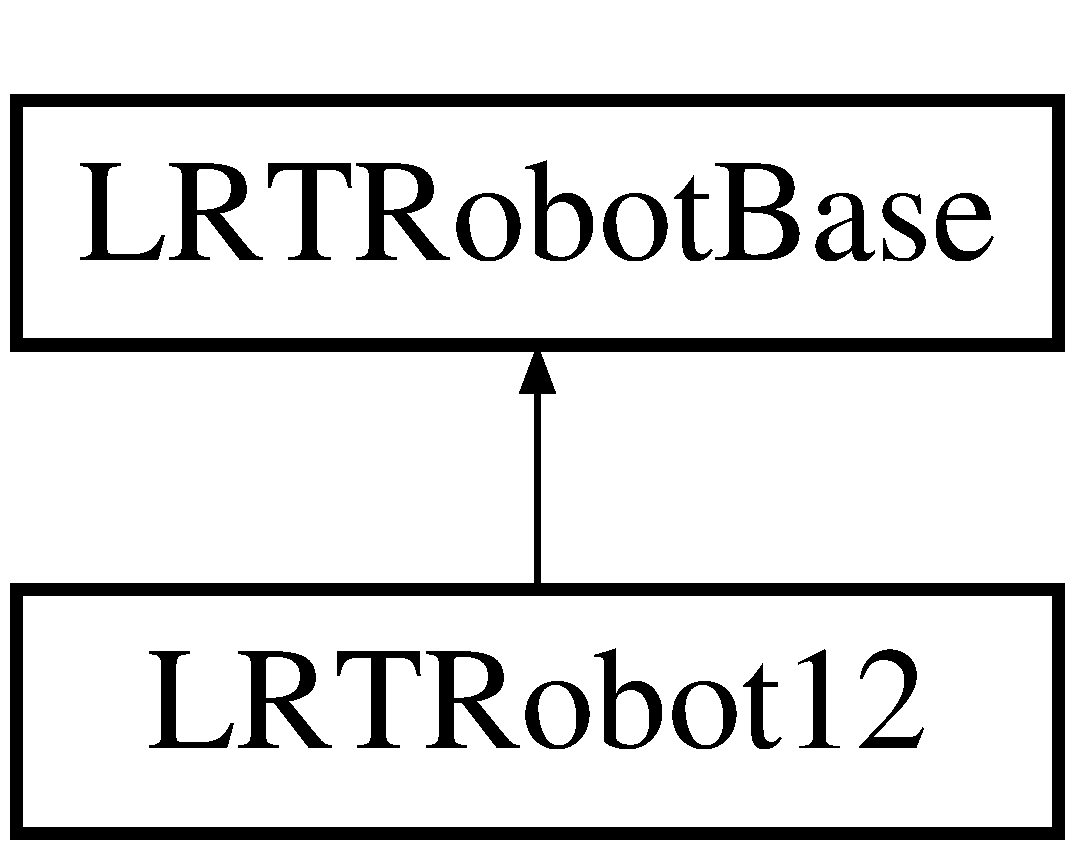
\includegraphics[height=2.000000cm]{class_l_r_t_robot12}
\end{center}
\end{figure}
\subsection*{\-Public \-Member \-Functions}
\begin{DoxyCompactItemize}
\item 
\hypertarget{class_l_r_t_robot12_a39758ff301b0112b74cefa7b10b11cbb}{virtual void {\bfseries \-Robot\-Init} ()}\label{class_l_r_t_robot12_a39758ff301b0112b74cefa7b10b11cbb}

\item 
\hypertarget{class_l_r_t_robot12_a43c496f6794d0d790857aea01e77791e}{virtual void {\bfseries \-Main\-Loop} ()}\label{class_l_r_t_robot12_a43c496f6794d0d790857aea01e77791e}

\end{DoxyCompactItemize}
\subsection*{\-Public \-Attributes}
\begin{DoxyCompactItemize}
\item 
\hypertarget{class_l_r_t_robot12_a6cc4a4daa8750d97f8f0da24361578a1}{\hyperlink{class_print_in_constructor}{\-Print\-In\-Constructor} {\bfseries first\-Member\-\_\-}}\label{class_l_r_t_robot12_a6cc4a4daa8750d97f8f0da24361578a1}

\end{DoxyCompactItemize}


\-The documentation for this class was generated from the following files\-:\begin{DoxyCompactItemize}
\item 
\-L\-R\-T\-Robot12.\-h\item 
\-L\-R\-T\-Robot12.\-cpp\end{DoxyCompactItemize}

\hypertarget{class_l_r_t_robot_base}{\section{\-L\-R\-T\-Robot\-Base \-Class \-Reference}
\label{class_l_r_t_robot_base}\index{\-L\-R\-T\-Robot\-Base@{\-L\-R\-T\-Robot\-Base}}
}
\-Inheritance diagram for \-L\-R\-T\-Robot\-Base\-:\begin{figure}[H]
\begin{center}
\leavevmode
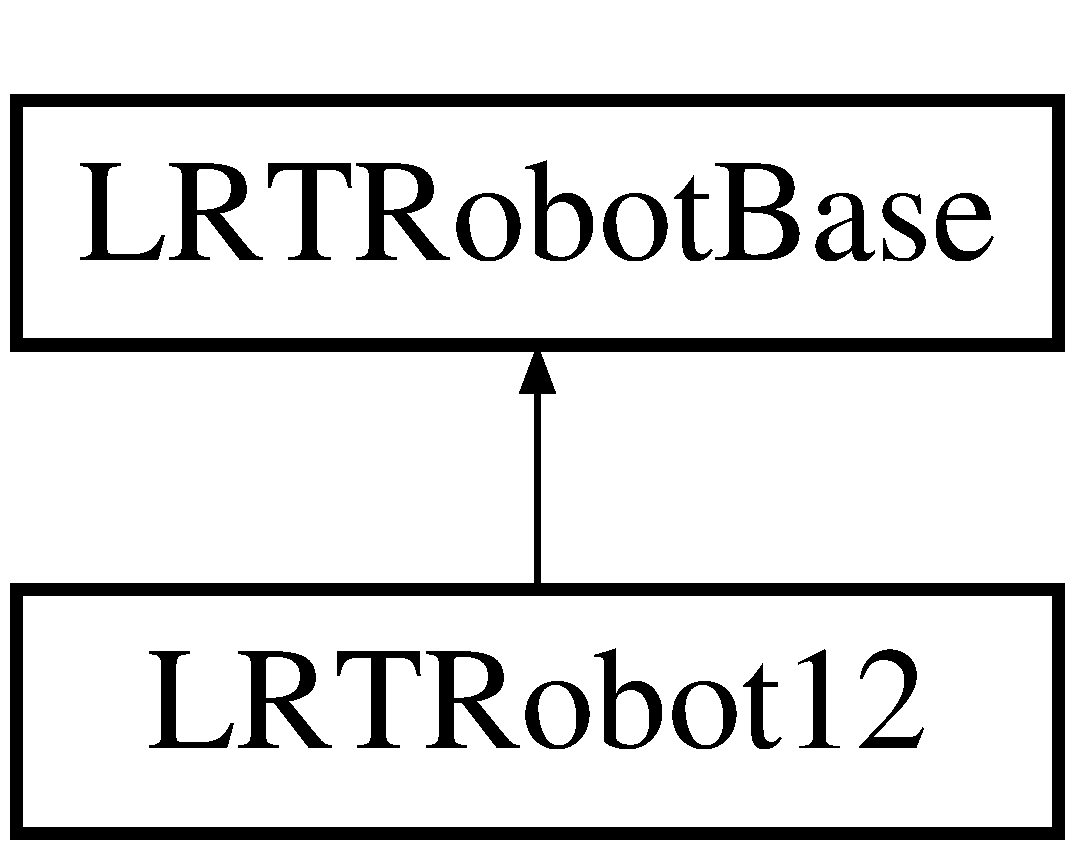
\includegraphics[height=2.000000cm]{class_l_r_t_robot_base}
\end{center}
\end{figure}
\subsection*{\-Public \-Member \-Functions}
\begin{DoxyCompactItemize}
\item 
virtual void \hyperlink{class_l_r_t_robot_base_a242e46650b04f58baaa6c3c585a15634}{\-Start\-Competition} ()
\item 
\hypertarget{class_l_r_t_robot_base_a8c1344352ad07a31cb4813433d2a30f1}{virtual void {\bfseries \-Robot\-Init} ()=0}\label{class_l_r_t_robot_base_a8c1344352ad07a31cb4813433d2a30f1}

\item 
\hypertarget{class_l_r_t_robot_base_af9508c789c4fe6248e327f0e4a853834}{virtual void {\bfseries \-Main\-Loop} ()=0}\label{class_l_r_t_robot_base_af9508c789c4fe6248e327f0e4a853834}

\end{DoxyCompactItemize}
\subsection*{\-Protected \-Member \-Functions}
\begin{DoxyCompactItemize}
\item 
\hyperlink{class_l_r_t_robot_base_a30dd1efa256483acec95edfd56435231}{\-L\-R\-T\-Robot\-Base} ()
\item 
virtual \hyperlink{class_l_r_t_robot_base_af12bef7e14e5f661b4c86f9d63158db2}{$\sim$\-L\-R\-T\-Robot\-Base} ()
\end{DoxyCompactItemize}
\subsection*{\-Protected \-Attributes}
\begin{DoxyCompactItemize}
\item 
\hypertarget{class_l_r_t_robot_base_a034106e704c8c9c1dba6b582c8181a40}{bool {\bfseries quitting\-\_\-}}\label{class_l_r_t_robot_base_a034106e704c8c9c1dba6b582c8181a40}

\item 
\hypertarget{class_l_r_t_robot_base_aea6cb7f9036013e76242d06912443bcd}{int {\bfseries cycle\-Count}}\label{class_l_r_t_robot_base_aea6cb7f9036013e76242d06912443bcd}

\item 
\hypertarget{class_l_r_t_robot_base_a45e2e098ce344d03e1e7a0862139d962}{int {\bfseries packets\-Missed\-In\-Lifetime}}\label{class_l_r_t_robot_base_a45e2e098ce344d03e1e7a0862139d962}

\end{DoxyCompactItemize}


\subsection{\-Constructor \& \-Destructor \-Documentation}
\hypertarget{class_l_r_t_robot_base_a30dd1efa256483acec95edfd56435231}{\index{\-L\-R\-T\-Robot\-Base@{\-L\-R\-T\-Robot\-Base}!\-L\-R\-T\-Robot\-Base@{\-L\-R\-T\-Robot\-Base}}
\index{\-L\-R\-T\-Robot\-Base@{\-L\-R\-T\-Robot\-Base}!LRTRobotBase@{\-L\-R\-T\-Robot\-Base}}
\subsubsection[{\-L\-R\-T\-Robot\-Base}]{\setlength{\rightskip}{0pt plus 5cm}{\bf \-L\-R\-T\-Robot\-Base\-::\-L\-R\-T\-Robot\-Base} (
\begin{DoxyParamCaption}
{}
\end{DoxyParamCaption}
)\hspace{0.3cm}{\ttfamily  \mbox{[}protected\mbox{]}}}}\label{class_l_r_t_robot_base_a30dd1efa256483acec95edfd56435231}
\-Constructor for \-Robot\-Iterative\-Base. \-Initializes member variables. \hypertarget{class_l_r_t_robot_base_af12bef7e14e5f661b4c86f9d63158db2}{\index{\-L\-R\-T\-Robot\-Base@{\-L\-R\-T\-Robot\-Base}!$\sim$\-L\-R\-T\-Robot\-Base@{$\sim$\-L\-R\-T\-Robot\-Base}}
\index{$\sim$\-L\-R\-T\-Robot\-Base@{$\sim$\-L\-R\-T\-Robot\-Base}!LRTRobotBase@{\-L\-R\-T\-Robot\-Base}}
\subsubsection[{$\sim$\-L\-R\-T\-Robot\-Base}]{\setlength{\rightskip}{0pt plus 5cm}{\bf \-L\-R\-T\-Robot\-Base\-::$\sim$\-L\-R\-T\-Robot\-Base} (
\begin{DoxyParamCaption}
{}
\end{DoxyParamCaption}
)\hspace{0.3cm}{\ttfamily  \mbox{[}protected, virtual\mbox{]}}}}\label{class_l_r_t_robot_base_af12bef7e14e5f661b4c86f9d63158db2}
\-Free the resources for a \-Robot\-Iterative\-Base class. 

\subsection{\-Member \-Function \-Documentation}
\hypertarget{class_l_r_t_robot_base_a242e46650b04f58baaa6c3c585a15634}{\index{\-L\-R\-T\-Robot\-Base@{\-L\-R\-T\-Robot\-Base}!\-Start\-Competition@{\-Start\-Competition}}
\index{\-Start\-Competition@{\-Start\-Competition}!LRTRobotBase@{\-L\-R\-T\-Robot\-Base}}
\subsubsection[{\-Start\-Competition}]{\setlength{\rightskip}{0pt plus 5cm}void {\bf \-L\-R\-T\-Robot\-Base\-::\-Start\-Competition} (
\begin{DoxyParamCaption}
{}
\end{DoxyParamCaption}
)\hspace{0.3cm}{\ttfamily  \mbox{[}virtual\mbox{]}}}}\label{class_l_r_t_robot_base_a242e46650b04f58baaa6c3c585a15634}
\-Used to continuously call the \-Main\-Loop method while printing diagnostics. 

\-The documentation for this class was generated from the following files\-:\begin{DoxyCompactItemize}
\item 
\-L\-R\-T\-Robot\-Base.\-h\item 
\-L\-R\-T\-Robot\-Base.\-cpp\end{DoxyCompactItemize}

\hypertarget{class_print_in_constructor}{\section{\-Print\-In\-Constructor \-Class \-Reference}
\label{class_print_in_constructor}\index{\-Print\-In\-Constructor@{\-Print\-In\-Constructor}}
}
\subsection*{\-Public \-Member \-Functions}
\begin{DoxyCompactItemize}
\item 
\hypertarget{class_print_in_constructor_a325bfa0ad054243598783a66efe62929}{{\bfseries \-Print\-In\-Constructor} (const char $\ast$ctor\-\_\-dtor\-\_\-message)}\label{class_print_in_constructor_a325bfa0ad054243598783a66efe62929}

\item 
\hypertarget{class_print_in_constructor_abbb5d38c5df27a4329c32b4855d5314c}{{\bfseries \-Print\-In\-Constructor} (const char $\ast$ctor\-\_\-message, const char $\ast$dtor\-\_\-message)}\label{class_print_in_constructor_abbb5d38c5df27a4329c32b4855d5314c}

\end{DoxyCompactItemize}
\subsection*{\-Public \-Attributes}
\begin{DoxyCompactItemize}
\item 
\hypertarget{class_print_in_constructor_a1309cc9a11057725be496b726de64264}{std\-::string {\bfseries destructor\-Message\-\_\-}}\label{class_print_in_constructor_a1309cc9a11057725be496b726de64264}

\end{DoxyCompactItemize}
\subsection*{\-Protected \-Member \-Functions}
\begin{DoxyCompactItemize}
\item 
\hypertarget{class_print_in_constructor_a92a3e887114ae3ee7cacbb2196f8279e}{void {\bfseries \-Initialize} (const char $\ast$ctor\-\_\-message, const char $\ast$dtor\-\_\-message)}\label{class_print_in_constructor_a92a3e887114ae3ee7cacbb2196f8279e}

\end{DoxyCompactItemize}


\-The documentation for this class was generated from the following files\-:\begin{DoxyCompactItemize}
\item 
\-Util/\-Print\-In\-Constructor.\-h\item 
\-Util/\-Print\-In\-Constructor.\-cpp\end{DoxyCompactItemize}

\hypertarget{class_profiled_section}{\section{\-Profiled\-Section \-Class \-Reference}
\label{class_profiled_section}\index{\-Profiled\-Section@{\-Profiled\-Section}}
}
\subsection*{\-Public \-Member \-Functions}
\begin{DoxyCompactItemize}
\item 
\hypertarget{class_profiled_section_a19f4ad2ae1f348309f0d5169fea83e57}{{\bfseries \-Profiled\-Section} (std\-::string name)}\label{class_profiled_section_a19f4ad2ae1f348309f0d5169fea83e57}

\end{DoxyCompactItemize}
\subsection*{\-Protected \-Attributes}
\begin{DoxyCompactItemize}
\item 
\hypertarget{class_profiled_section_ae02896dd4964d227e3557dd47387580f}{string {\bfseries name}}\label{class_profiled_section_ae02896dd4964d227e3557dd47387580f}

\item 
\hypertarget{class_profiled_section_a36b51e1d06631a8b00ecd587bc236165}{double {\bfseries start}}\label{class_profiled_section_a36b51e1d06631a8b00ecd587bc236165}

\end{DoxyCompactItemize}


\-The documentation for this class was generated from the following file\-:\begin{DoxyCompactItemize}
\item 
\-Util/\-Profiler.\-h\end{DoxyCompactItemize}

\hypertarget{class_profiler}{\section{\-Profiler \-Class \-Reference}
\label{class_profiler}\index{\-Profiler@{\-Profiler}}
}


{\ttfamily \#include $<$\-Profiler.\-h$>$}

\subsection*{\-Public \-Member \-Functions}
\begin{DoxyCompactItemize}
\item 
\hypertarget{class_profiler_a5953010288cfb36c95e84f0370411cbc}{void {\bfseries \-Start\-New\-Cycle} ()}\label{class_profiler_a5953010288cfb36c95e84f0370411cbc}

\item 
\hypertarget{class_profiler_a9baecdda5cc00bd43d6196105d34ce32}{void {\bfseries \-Log} (std\-::string name, double time\-Taken)}\label{class_profiler_a9baecdda5cc00bd43d6196105d34ce32}

\item 
\hypertarget{class_profiler_afea0a7425697009c14fb240ada89a37b}{void {\bfseries \-Clear\-Log\-Buffer} ()}\label{class_profiler_afea0a7425697009c14fb240ada89a37b}

\end{DoxyCompactItemize}
\subsection*{\-Static \-Public \-Member \-Functions}
\begin{DoxyCompactItemize}
\item 
\hypertarget{class_profiler_a97ff2f7bcb63ca90750389049f7038a3}{static \hyperlink{class_profiler}{\-Profiler} \& {\bfseries \-Get\-Instance} ()}\label{class_profiler_a97ff2f7bcb63ca90750389049f7038a3}

\end{DoxyCompactItemize}
\subsection*{\-Static \-Public \-Attributes}
\begin{DoxyCompactItemize}
\item 
\hypertarget{class_profiler_a7c1def2ecb10a5400799769ae2c5b6eb}{static const int {\bfseries report\-Period} = 50 $\ast$ 5}\label{class_profiler_a7c1def2ecb10a5400799769ae2c5b6eb}

\item 
\hypertarget{class_profiler_a28a468656e52f8bbeaf2a76c07ecdac2}{static const int {\bfseries report\-Limit} = 10}\label{class_profiler_a28a468656e52f8bbeaf2a76c07ecdac2}

\end{DoxyCompactItemize}
\subsection*{\-Protected \-Member \-Functions}
\begin{DoxyCompactItemize}
\item 
\hypertarget{class_profiler_aea7082b3ac45f3e77f163e7647c03b67}{{\bfseries \-D\-I\-S\-A\-L\-L\-O\-W\-\_\-\-C\-O\-P\-Y\-\_\-\-A\-N\-D\-\_\-\-A\-S\-S\-I\-G\-N} (\hyperlink{class_profiler}{\-Profiler})}\label{class_profiler_aea7082b3ac45f3e77f163e7647c03b67}

\end{DoxyCompactItemize}


\subsection{\-Detailed \-Description}
\-Usage\-:

\{ \hyperlink{class_profiled_section}{\-Profiled\-Section} pf( \char`\"{}\-Name\-Of\-Activity\char`\"{} ); // do something time consuming... \} 

\-The documentation for this class was generated from the following files\-:\begin{DoxyCompactItemize}
\item 
\-Util/\-Profiler.\-h\item 
\-Util/\-Profiler.\-cpp\end{DoxyCompactItemize}

\hypertarget{class_profiler_helper}{\section{\-Profiler\-Helper \-Class \-Reference}
\label{class_profiler_helper}\index{\-Profiler\-Helper@{\-Profiler\-Helper}}
}
\subsection*{\-Public \-Member \-Functions}
\begin{DoxyCompactItemize}
\item 
\hypertarget{class_profiler_helper_a08d89456f48b8d2e4b5239dcfa7527a1}{void {\bfseries \-Start} (string name)}\label{class_profiler_helper_a08d89456f48b8d2e4b5239dcfa7527a1}

\item 
\hypertarget{class_profiler_helper_a5e125e2c8280418c539269438e97568a}{void {\bfseries \-Finish} ()}\label{class_profiler_helper_a5e125e2c8280418c539269438e97568a}

\end{DoxyCompactItemize}
\subsection*{\-Protected \-Attributes}
\begin{DoxyCompactItemize}
\item 
\hypertarget{class_profiler_helper_a6676fb76738693e3c0cb628ca43de7f1}{string {\bfseries name}}\label{class_profiler_helper_a6676fb76738693e3c0cb628ca43de7f1}

\item 
\hypertarget{class_profiler_helper_a624a70218836e1560374ba9dc386624a}{double {\bfseries start}}\label{class_profiler_helper_a624a70218836e1560374ba9dc386624a}

\end{DoxyCompactItemize}


\-The documentation for this class was generated from the following file\-:\begin{DoxyCompactItemize}
\item 
\-Util/\-Profiler.\-h\end{DoxyCompactItemize}

\hypertarget{class_running_sum}{\section{\-Running\-Sum \-Class \-Reference}
\label{class_running_sum}\index{\-Running\-Sum@{\-Running\-Sum}}
}
\subsection*{\-Public \-Member \-Functions}
\begin{DoxyCompactItemize}
\item 
\hypertarget{class_running_sum_a3ef30833e073d096a2561bad579139b3}{{\bfseries \-Running\-Sum} (float decay\-Constant)}\label{class_running_sum_a3ef30833e073d096a2561bad579139b3}

\item 
\hypertarget{class_running_sum_a2ce3ef61ad0966adc167f499bbd676a9}{float {\bfseries \-Update\-Sum} (float x)}\label{class_running_sum_a2ce3ef61ad0966adc167f499bbd676a9}

\item 
\hypertarget{class_running_sum_a6e3d39b38161f01979275007b518abb5}{void {\bfseries \-Clear} ()}\label{class_running_sum_a6e3d39b38161f01979275007b518abb5}

\end{DoxyCompactItemize}


\-The documentation for this class was generated from the following file\-:\begin{DoxyCompactItemize}
\item 
\-Util/\-Running\-Sum.\-h\end{DoxyCompactItemize}

\hypertarget{struct_sort_by_second_value}{\section{\-Sort\-By\-Second\-Value$<$ \-Pair\-T $>$ \-Struct \-Template \-Reference}
\label{struct_sort_by_second_value}\index{\-Sort\-By\-Second\-Value$<$ Pair\-T $>$@{\-Sort\-By\-Second\-Value$<$ Pair\-T $>$}}
}
\subsection*{\-Public \-Member \-Functions}
\begin{DoxyCompactItemize}
\item 
\hypertarget{struct_sort_by_second_value_ab275494b78541d6c37f54597d4824980}{bool {\bfseries operator()} (const \-Pair\-T \&lhs, const \-Pair\-T \&rhs) const }\label{struct_sort_by_second_value_ab275494b78541d6c37f54597d4824980}

\end{DoxyCompactItemize}
\subsubsection*{template$<$class Pair\-T$>$ struct Sort\-By\-Second\-Value$<$ Pair\-T $>$}



\-The documentation for this struct was generated from the following file\-:\begin{DoxyCompactItemize}
\item 
\-Util/\-Profiler.\-cpp\end{DoxyCompactItemize}

\hypertarget{class_util}{\section{\-Util \-Class \-Reference}
\label{class_util}\index{\-Util@{\-Util}}
}
\subsection*{\-Static \-Public \-Member \-Functions}
\begin{DoxyCompactItemize}
\item 
\hypertarget{class_util_ae96fb04ebf846f501ebd96d7455027a9}{{\footnotesize template$<$typename T $>$ }\\static \-T {\bfseries \-Clamp} (\-T val, \-T min, \-T max)}\label{class_util_ae96fb04ebf846f501ebd96d7455027a9}

\item 
\hypertarget{class_util_a104bdc57a1eba1e8863f8139985e9b05}{{\footnotesize template$<$typename T $>$ }\\static \-T {\bfseries \-Rescale} (\-T val, \-T min0, \-T max0, \-T min1, \-T max1)}\label{class_util_a104bdc57a1eba1e8863f8139985e9b05}

\item 
\hypertarget{class_util_a120427fa00fd2e48bcc5b48088aeef84}{{\footnotesize template$<$typename T $>$ }\\static std\-::string {\bfseries \-To\-String} (\-T val)}\label{class_util_a120427fa00fd2e48bcc5b48088aeef84}

\item 
\hypertarget{class_util_ae608455719c51e7478f56a1366f50a1e}{{\footnotesize template$<$typename T $>$ }\\static int {\bfseries \-Sign} (\-T val)}\label{class_util_ae608455719c51e7478f56a1366f50a1e}

\item 
\hypertarget{class_util_a1e847664f26f1a545b1c8414ec8bbc90}{{\footnotesize template$<$typename T $>$ }\\static \-T {\bfseries \-Abs} (\-T val)}\label{class_util_a1e847664f26f1a545b1c8414ec8bbc90}

\item 
\hypertarget{class_util_a2a09028ede419c2da1f1e308fa811a73}{{\footnotesize template$<$typename T $>$ }\\static void {\bfseries \-Min\-Max\-Mean} (\-T val\mbox{[}$\,$\mbox{]}, int n, \-T $\ast$min\-Out, \-T $\ast$max\-Out, \-T $\ast$mean\-Out)}\label{class_util_a2a09028ede419c2da1f1e308fa811a73}

\item 
\hypertarget{class_util_afc2afb1ef9fcc6f47277931ffe26b421}{{\footnotesize template$<$typename T $>$ }\\static \-T {\bfseries \-Add\-Deadband} (\-T raw, \-T deadband\-Size)}\label{class_util_afc2afb1ef9fcc6f47277931ffe26b421}

\item 
\hypertarget{class_util_ad81fcab61c9cbcbea59a61e68e77ba60}{{\footnotesize template$<$typename T $>$ }\\static \-T {\bfseries \-Val\-With\-Abs\-Max} (\-T val1, \-T val2)}\label{class_util_ad81fcab61c9cbcbea59a61e68e77ba60}

\item 
\hypertarget{class_util_a8430d16e2dde9becfe7f6f22f0ed82bf}{{\footnotesize template$<$typename T $>$ }\\static \-T {\bfseries \-Max} (\-T val1, \-T val2)}\label{class_util_a8430d16e2dde9becfe7f6f22f0ed82bf}

\item 
\hypertarget{class_util_a58c0162c35e293d94f8fdfe5df4f8df9}{{\footnotesize template$<$typename T $>$ }\\static \-T {\bfseries \-Min} (\-T val1, \-T val2)}\label{class_util_a58c0162c35e293d94f8fdfe5df4f8df9}

\item 
\hypertarget{class_util_adf538ad330a0b0962a49b2692d777df2}{{\footnotesize template$<$typename T $>$ }\\static \-T {\bfseries \-Pow\-Preseve\-Sign} (\-T val, int power)}\label{class_util_adf538ad330a0b0962a49b2692d777df2}

\item 
\hypertarget{class_util_ace9563b1a67ff4f43c95aafda00978d0}{static void {\bfseries \-Die} ()}\label{class_util_ace9563b1a67ff4f43c95aafda00978d0}

\item 
\hypertarget{class_util_a1ad96657e2a363fb601d058d14d5e9d8}{static void {\bfseries \-Die} (const char $\ast$message)}\label{class_util_a1ad96657e2a363fb601d058d14d5e9d8}

\item 
\hypertarget{class_util_a49e0d861927bda16820e16dda8dfdc74}{static bool {\bfseries \-Assert} (bool test, const char $\ast$message)}\label{class_util_a49e0d861927bda16820e16dda8dfdc74}

\end{DoxyCompactItemize}


\-The documentation for this class was generated from the following files\-:\begin{DoxyCompactItemize}
\item 
\-Util/\-Util.\-h\item 
\-Util/\-Util.\-cpp\end{DoxyCompactItemize}

\printindex
\end{document}
